\documentclass{sig-alternate}
%\usepackage{color}
%\usepackage[colorinlistoftodos]{todonotes}
\usepackage{graphicx}

%%%%% Uncomment the following line and comment out the previous one
%%%%% to remove all comments
%%%%% NOTE: comments still occupy a line even if invisible;
%%%%% Don't write them as a separate paragraph
%\newcommand{\mycomment}[1]{}

\begin{document}

% --- Author Metadata here ---
%%% REMEMBER TO CHANGE THE SEMESTER AND YEAR
\conferenceinfo{UMM CSci Senior Seminar Conference, April 2014}{Morris, MN}

\title{Morphological Operations Applied to Crack Detection in Digital Art Restoration}

\numberofauthors{1}

\author{
% The command \alignauthor (no curly braces needed) should
% precede each author name, affiliation/snail-mail address and
% e-mail address. Additionally, tag each line of
% affiliation/address with \affaddr, and tag the
% e-mail address with \email.
\alignauthor
M. Kirbie Dramdahl\\
	\affaddr{Division of Science and Mathematics}\\
	\affaddr{University of Minnesota, Morris}\\
	\affaddr{Morris, Minnesota, USA 56267}\\
	\email{dramd002@morris.umn.edu}
}

\maketitle
\begin{abstract}
\end{abstract}

%\category

%\terms

%\keywords

\section{Introduction}

\section{Edge Detection}\label{edge detection}

\section{Morphological Operations}
Mathematical morphology is an area of set theory, and a method of image processing. Typically, it is used in processing binary (black and white) images, although there are also variations used for gray scale images. Here, we will focus on binary images. Morphological functions take two inputs. The first input is the image to be processed, divided into foreground (typically white) and background (typically black) regions. The second input is a structuring element, a (typically small, in comparison to the image) set of coordinate points. The structuring element is then used to modify the input image. The image that results from the morphological operation is determined by the shape, size, and point of origin of the structuring element \cite{MorphologyWikiAnonymous, MorphologyBook:2000, MorphologyWiki, MorphologyPaper:1987}. Subsections \ref{erosion}, \ref{dilation}, \ref{opening}, and \ref{closing} explain the fundamental operations of mathematical morphology.

\subsection{Erosion}\label{erosion}
Erosion of an image strips away a layer of pixels from the boundaries of foreground regions, and is denoted by the equation
\begin{equation*}
g = f \ominus s
\end{equation*}
where \textit{g} is the resulting image, \textit{f} is the original image, and \textit{s} is the structuring element \cite{MorphologyWikiAnonymous, MorphologyBook:2000}. This is accomplished by placing the origin of the structuring element over every pixel of the foreground regions in turn. If every point within the structuring element is in line with a foreground pixel, the foreground pixel lined up with the origin of the structuring element is left unchanged. If at least one point within the structuring element is in line with a background pixel, then the pixel lined up with the origin of the structuring element is converted to a background pixel \cite{MorphologyWiki}. An example of erosion using a 3x3 square structuring element with the origin located at the center is presented in Figure 1. The erosion of foreground regions is equivalent to the dilation (discussed in subsection \ref{dilation}) of background regions \cite{MorphologyWiki}.
\begin{figure}
\centering
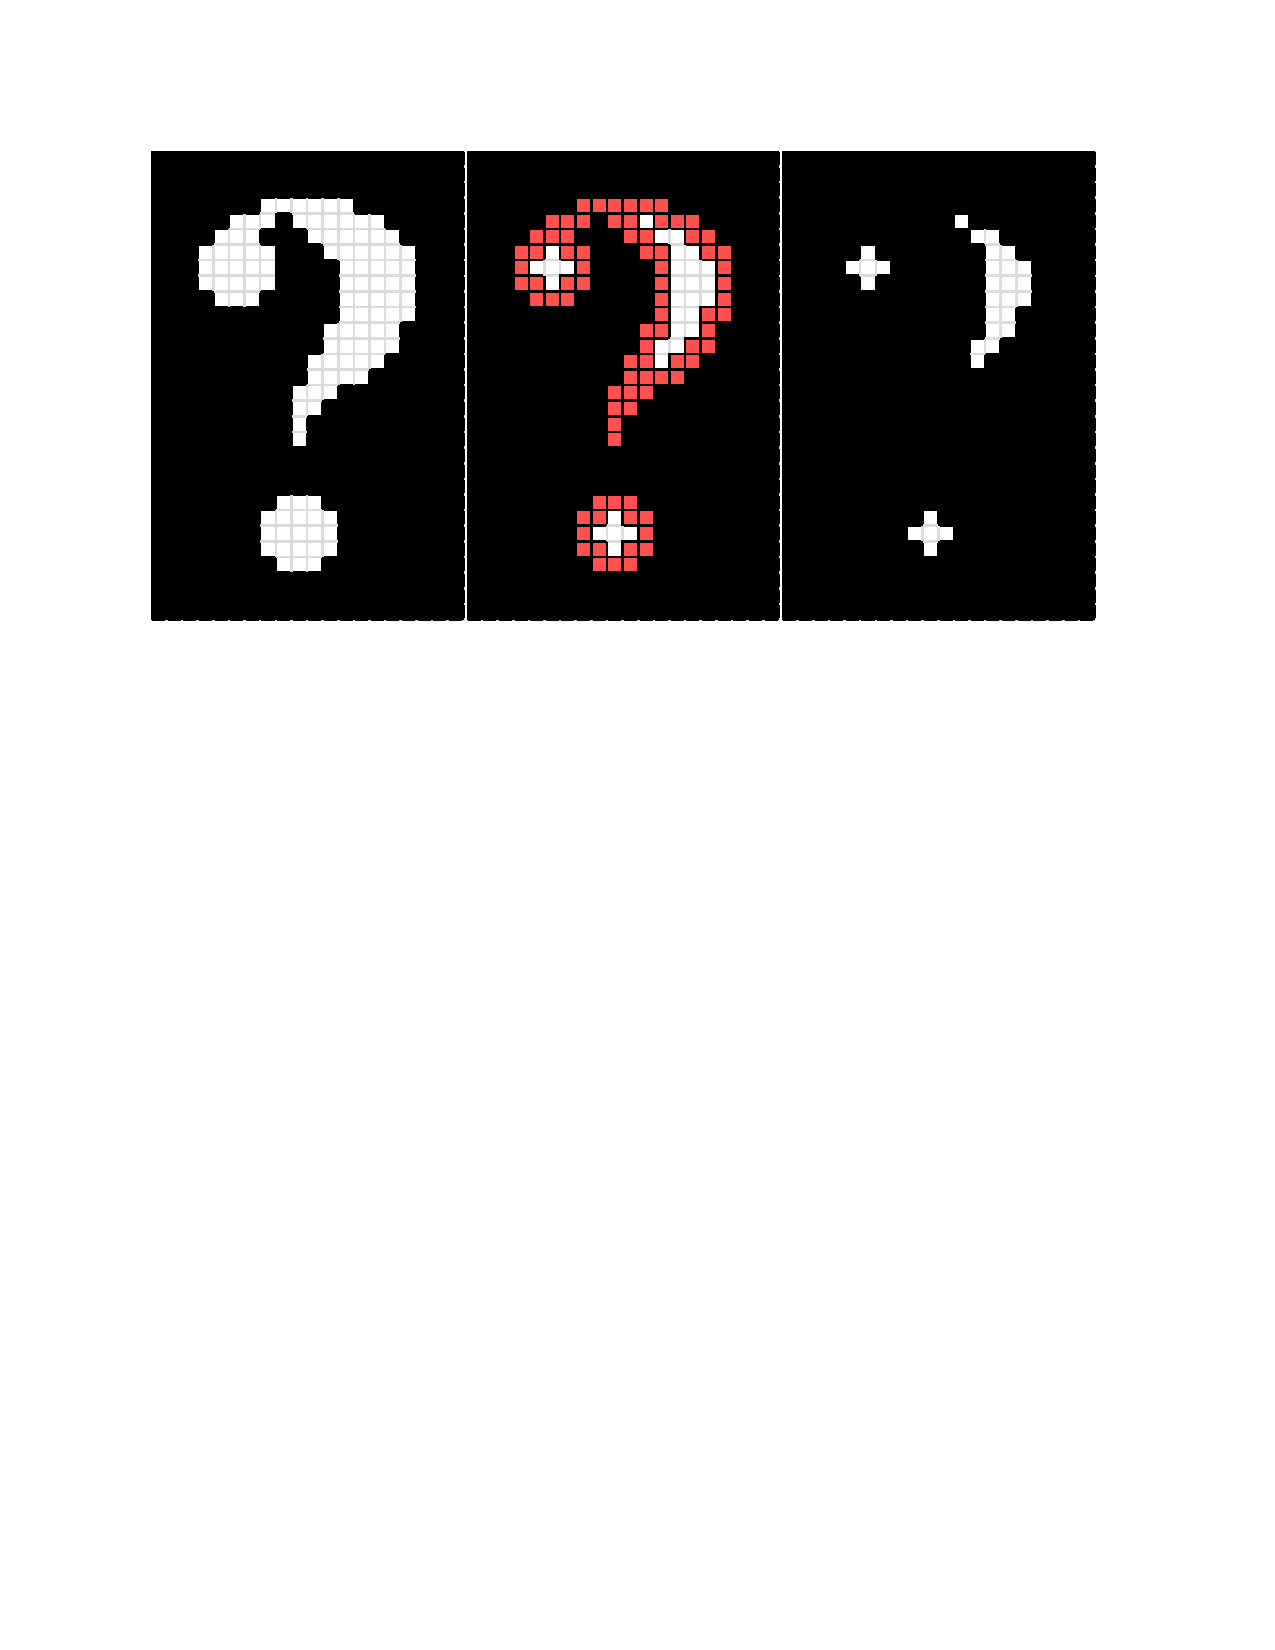
\includegraphics[width=3in,trim={0 6.75in 0 0},clip]{erosion}
\caption{Erosion: Left: Original Image. Center: Erosion Marked in Red. Right: Results of Erosion.}
\end{figure}

\subsection{Dilation}\label{dilation}
Dilation of an image adds a layer of pixels to the boundaries of foreground regions, and is denoted by the equation
\begin{equation*}
g = f \oplus s
\end{equation*}
where \textit{g} is the resulting image, \textit{f} is the original image, and \textit{s} is the structuring element \cite{MorphologyWikiAnonymous, MorphologyBook:2000}. This is accomplished by placing the origin of the structuring element over every pixel of the background regions in turn. If every point within the structuring element is in line with a background pixel, the background pixel lined up with the origin of the structuring element is left unchanged. If at least one point within the structuring element is in line with a foreground pixel, then the pixel lined up with the origin of the structuring element is converted to a foreground pixel \cite{MorphologyWiki}. An example of dilation using a 3x3 square structuring element with the origin located at the center is presented in Figure 2. The dilation of foreground regions is equivalent to the erosion (discussed in subsection \ref{erosion}) of background regions \cite{MorphologyWiki}.
\begin{figure}
\centering

\includegraphics[width=3in,trim={0 6.75in 0 0},clip]{dilation}
\caption{Dilation: Left: Original Image. Center: Dilation Marked in Green. Right: Results of Dilation.}
\end{figure}

\subsection{Opening}\label{opening}
Opening of an image is an erosion followed by a dilation, and is denoted by the equation
\begin{equation*}
g = f \circ s = (f \ominus s) \oplus s
\end{equation*}
where \textit{g} is the resulting image, \textit{f} is the original image, and \textit{s} is the structuring element \cite{MorphologyWikiAnonymous, MorphologyBook:2000}. Similar to erosion, opening strips away foreground pixels at the boundaries of foreground regions, but is less destructive of the initial foreground regions than erosion. Opening is therefore typically used to preserve foreground regions with a similar size and shape to the structuring element, while removing or reducing other foreground regions \cite{MorphologyWiki}. An example of opening using a 3x3 square structuring element with the origin located at the center is presented in Figure 3. Additionally, opening is idempotent, meaning that once an image has been opened, additional openings with the same structuring element will have no further effect on the image \cite{MorphologyWiki, MorphologyPaper:1987}. The idempotence of opening is denoted by the equation
\begin{equation*}
g = (f \circ s) \circ s = f \circ s
\end{equation*}
where, as before, \textit{g} is the resulting image, \textit{f} is the original image, and \textit{s} is the structuring element \cite{MorphologyWikiAnonymous}. The opening of foreground regions is equivalent to the closing of background regions \cite{MorphologyWiki}.
\begin{figure}
\centering
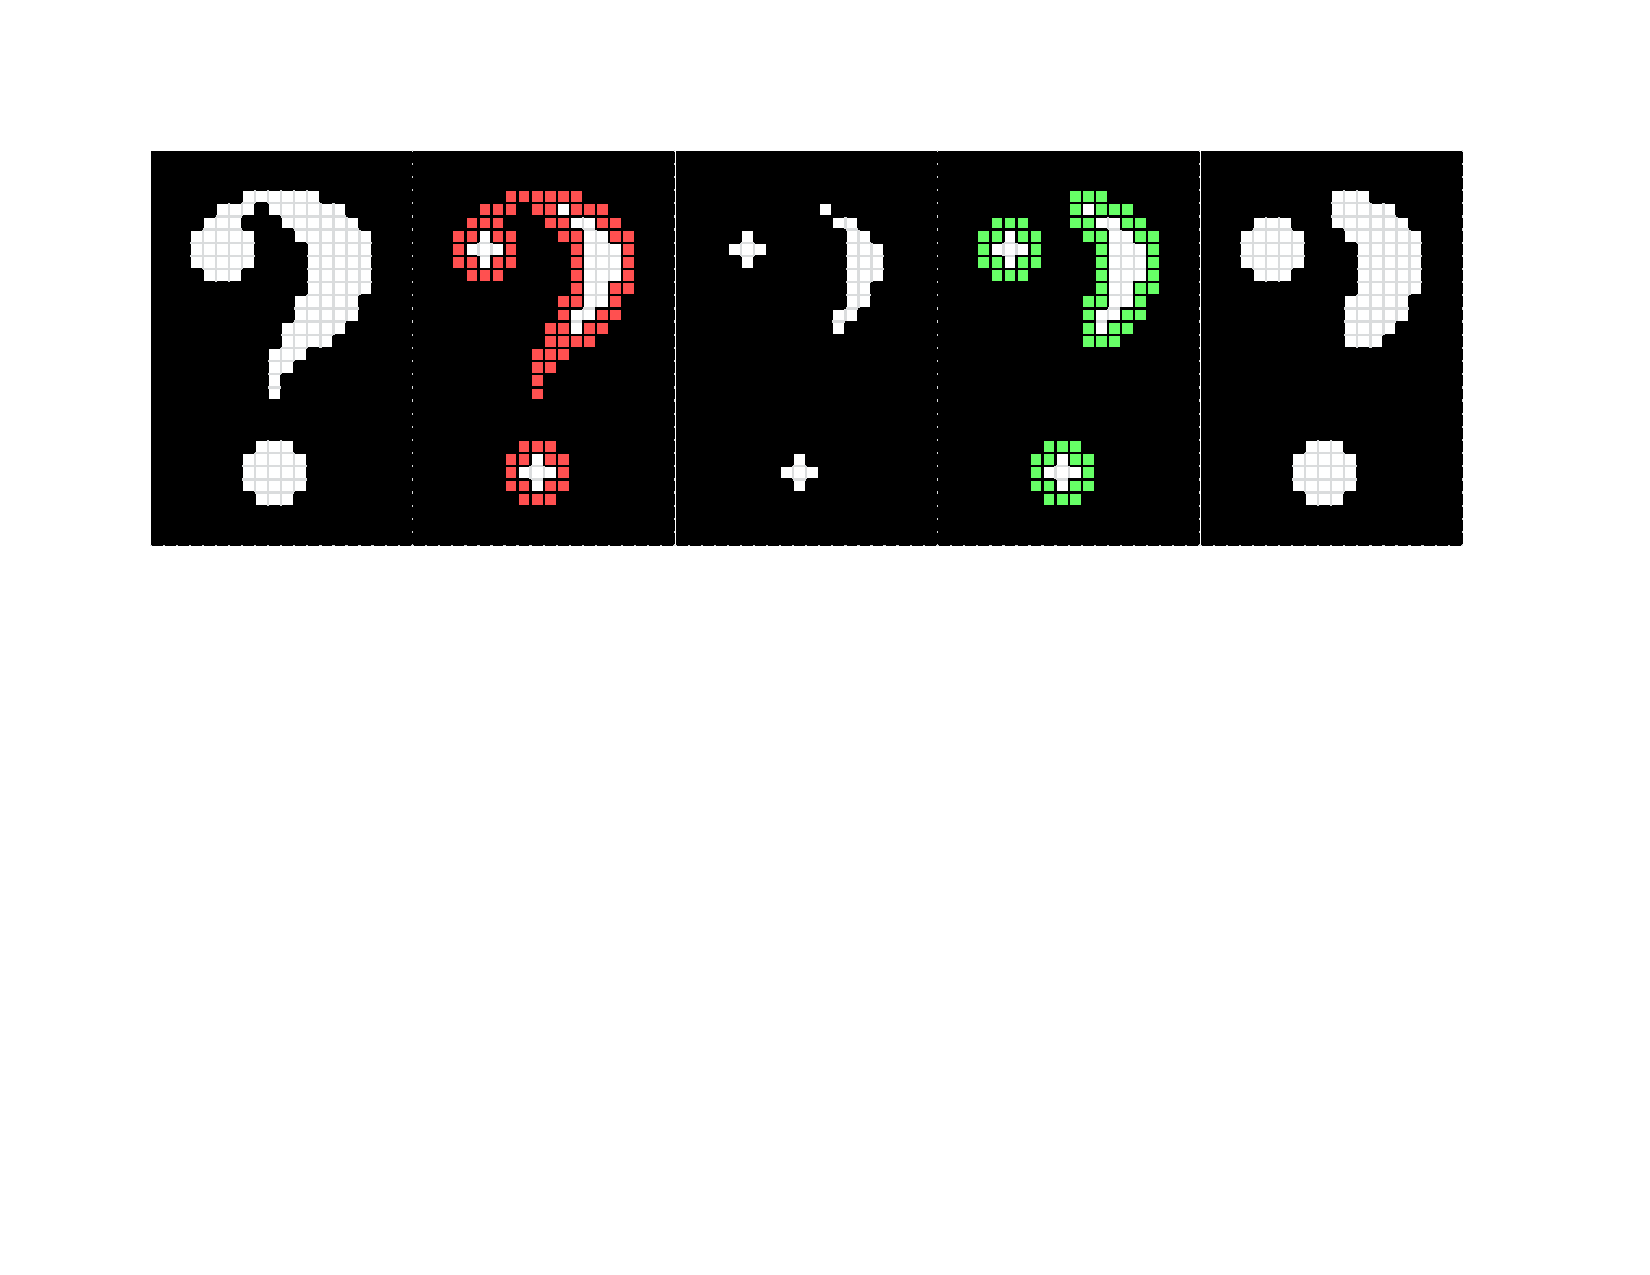
\includegraphics[width=3in,trim={0 4.75in 0 0},clip]{opening}
\caption{Opening: Left: Original Image. Second from Left: Erosion Marked in Red. Center: Results of Erosion. Second from Right: Dilation Marked in Green. Right: Results of Dilation (Opening Complete).}
\end{figure}

\subsection{Closing}\label{closing}
Closing of an image is a dilation followed by an erosion, and is denoted by the equation
\begin{equation*}
g = f \bullet s = (f \oplus s) \ominus s
\end{equation*}
where \textit{g} is the resulting image, \textit{f} is the original image, and \textit{s} is the structuring element \cite{MorphologyWikiAnonymous, MorphologyBook:2000}. Similar to dilation, closing adds foreground pixels at the boundaries of foreground regions, but is less destructive of the initial background regions than dilation. Closing is therefore typically used to preserve background regions with a similar size and shape to the structuring element, while removing or reducing other background regions \cite{MorphologyWiki}. An example of closing using a 3x3 square structuring element with the origin located at the center is presented in Figure 4. Additionally, closing is idempotent, meaning that once and image has been closed, additional closings with the same structuring element will have no further effect on the image \cite{MorphologyWiki, MorphologyPaper:1987}. The idempotence of closing is denoted by the equation
\begin{equation*}
g = (f \bullet s) \bullet s = f \bullet s
\end{equation*}
where, as before, \textit{g} is the resulting image, \textit{f} is the original image, and \textit{s} is the structuring element \cite{MorphologyWikiAnonymous}. The closing of foreground regions is equivalent to the opening of background regions \cite{MorphologyWiki}.
\begin{figure}
\centering

\includegraphics[width=3in,trim={0 4.75in 0 0},clip]{closing}
\caption{Closing: Left: Original Image. Second from Left: Dilation Marked in Green. Center: Results of Dilation. Second from Right: Erosion Marked in Red. Right: Results of Erosion (Closing Complete).}
\end{figure}

\section{Methods of Crack Detection}

\subsection{Top-Hat Transform}

\subsubsection{Black Top-Hat}\label{black top-hat}

\subsubsection{White Top-Hat}\label{white top-hat}

\subsubsection{Multiscale Top-Hat}

\subsection{Alternative Methods}

\section{Results}

\section{Conclusions}

\section{Acknowledgments}

% The following two commands are all you need in the
% initial runs of your .tex file to
% produce the bibliography for the citations in your paper.
\bibliographystyle{abbrv}
% sample_paper.bib is the name of the BibTex file containing the
% bibliography entries. Note that you *don't* include the .bib ending here.
\bibliography{morphology}  
% You must have a proper ".bib" file
%  and remember to run:
% latex bibtex latex latex
% to resolve all references

\end{document}